\subsubsection{Funkcjonalno��}

Okno wykres�w oferuje w pierwszej zak�adce podgl�d na pozycj� X-Y wszystkich robot�w dost�pnych na scenie. 

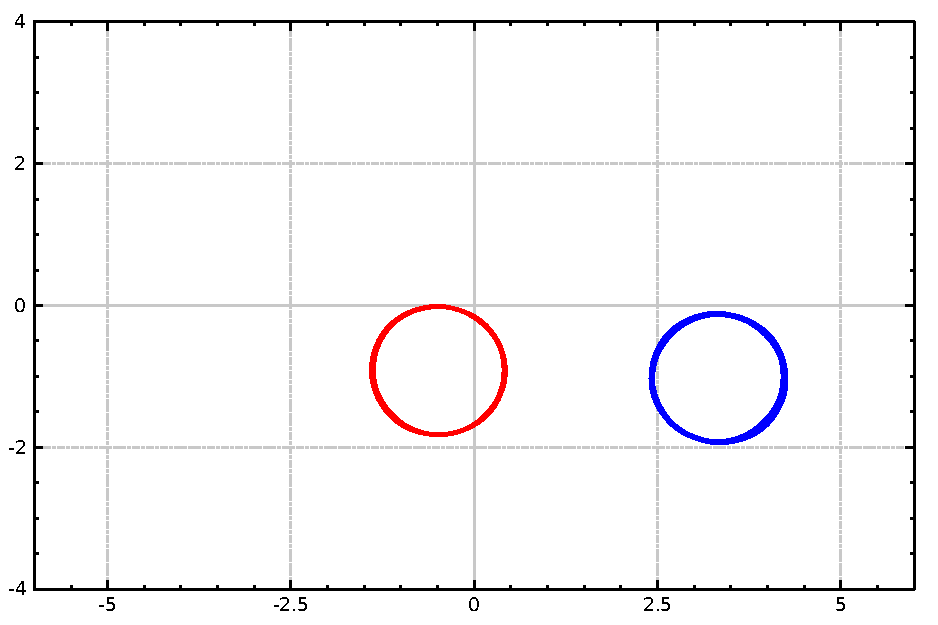
\includegraphics[height=5cm]{opis_systemu/wyniki_symulacji/images/robot_trace.pdf}

Na kolejnych wykresach ilustrowana jest pozycj� robota w osiach X,Y oraz orientacje wzgl�dem czasu symulacji.

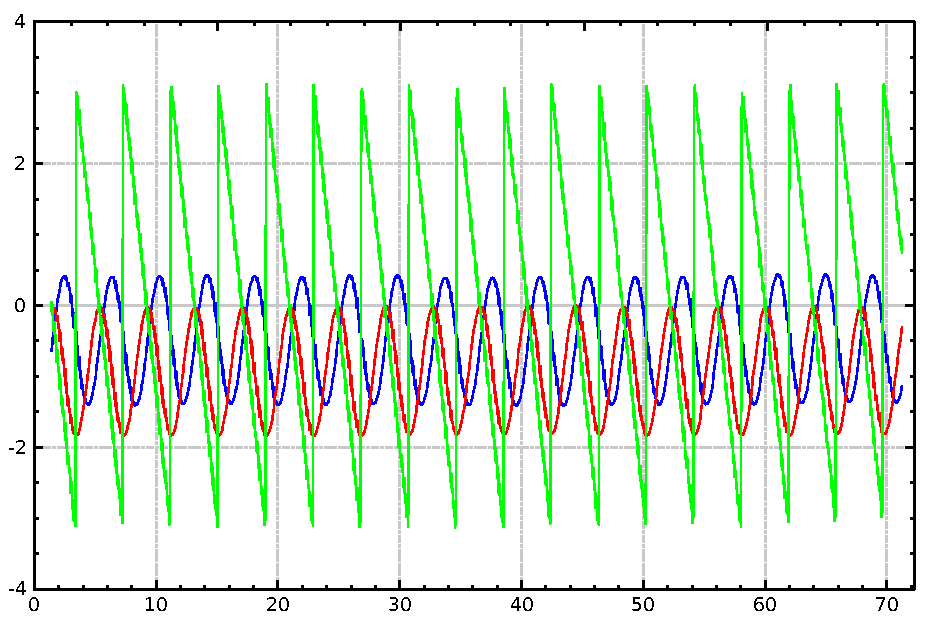
\includegraphics[height=5cm]{opis_systemu/wyniki_symulacji/images/robot_pose_2.pdf}

Okno zawiera dwa przyciski pozwalaj�ce na zresetowanie danych o robotach (czas symulacji nie zostaje zresetowany). Oraz przycisk pozwalaj�cy na zapis danych.

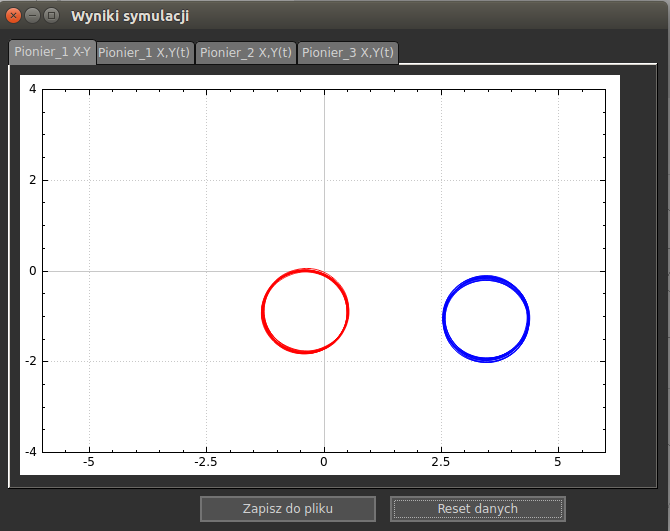
\includegraphics[height=5cm]{opis_systemu/wyniki_symulacji/images/zrzut_2.png}

Dane znajduj� si� w katalogu g��wnym kontenera. Wykresy s� zapisywane w postaci plik�w pdf. Program generuje r�wnie� plik csv z danymi uzyskanymi podczas symulacji. \\ \#Pionier1 X,Pionier1 Y,Pionier1 W,Pionier2 X,Pionier2 Y,Pionier2 W,Pionier3 X,Pionier3 Y,Pionier3 W,time\\
2.4122,-1.15,1.6118,-0.63934,-0.040688,0.047668,0,1,1,1.389\\
2.4082,-1.1215,1.5783,-0.61012,-0.036784,0.01829,0,0,0,1.409\\
2.4072,-1.1129,1.5685,-0.60134,-0.035781,0.0094779,0,0,0,1.415